\documentclass[10 pt,usenames,dvipsnames, oneside]{article}
\usepackage{../../../modelo-ensino-medio}



\begin{document}

\begin{center}
  \begin{minipage}[l]{3cm}

\includegraphics[width=2cm]{logo}    
\end{minipage}\hfill
\begin{minipage}[r]{.8\textwidth}
 {\Large \scshape Atividade: Dobradura}  
\end{minipage}
\end{center}
\vspace{.2cm}

\ifdefined\prof
%Habilidades da BNCC
\begin{objetivos}
\item \textbf{EM13MAT403} Comparar e analisar as representações, em plano cartesiano, das funções exponencial e logarítmica para identificar as características fundamentais (domínio, imagem, crescimento) de cada uma, com ou sem apoio de tecnologias digitais, estabelecendo relações entre elas.
\end{objetivos}

%Caixa do Para o Professor
\begin{goals}
%Objetivos específicos
\begin{enumerate}
	\item Reconhecer o padrão de decrescimento exponencial que aparece no experimento descrito;
	\item Identificar o fator de decrescimento e reconhecer o papel que ele desempenha na situação descrita.
\end{enumerate}

\tcblower

%Orientações e sugestões
\begin{itemize}
	\item Estimule os estudantes a realizarem o experimento.
\end{itemize}
\end{goals}

\bigskip
\begin{center}
{\large \scshape Atividade}
\end{center}
\fi

Uma folha de papel de área 1 é dobrada em três partes iguais, depois em mais três partes iguais, em terços novamente, e assim sucessivamente.

\begin{figure}[H]
\centering
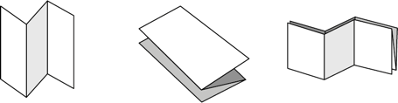
\includegraphics[width=250bp]{dobradura.png}
\end{figure}

\begin{enumerate}

\item{}
Na tabela abaixo registre a área da menor região em cada etapa, e o número total de regiões.

\begin{table}[H]
\centering

\begin{tabular}{|c|c|l|}
\hline
\tcolor{Etapas} & \tcolor{Área de cada região} & \tmcol{1}{c|}{Número de regiões} \\ \hline
0          &      1     & \multicolumn{1}{c|}{1}          \\ \hline
1          &           & \multicolumn{1}{c|}{}    \\ \hline
2          &           &                                 \\ \hline
3          &           &                                 \\ \hline
4          &           &                                 \\ \hline
5          &          &                                 \\ \hline
\end{tabular}
\end{table}

\item{}
Descreva os padrões observados na tabela e encontre uma expressão matemática que sirva para gerá-las em função das etapas.

\end{enumerate}

\ifdefined\prof
\begin{solucao}

\begin{enumerate}
	\item \adjustbox{valign=t}
	{\setlength\tabulinesep{2.5pt}
	\begin{tabu} to \textwidth{|c|c|c|}
	\hline
	\tcolor{Etapas} & \tcolor{Área de cada região} & \tmcol{1}{c|}{Número de regiões} \\ 
	\hline
	0 & $1$ & $1$ \\ 
	\hline
	1 & $\dfrac{1}{3}$ & $3$ \\ 
	\hline
	2 & $\dfrac{1}{9}$ & $9$ \\ 
	\hline
	3 & $\dfrac{1}{27}$ & $27$ \\ 
	\hline
	4 & $\dfrac{1}{81}$ & $81$ \\ 
	\hline
	5 & $\dfrac{1}{243}$ & $243$ \\ 
	\hline
	\end{tabu}
	}

	\item Em cada nova etapa a área da menor região é obtida dividindo por 3 a área da menor região da etapa anterior, já o número de regiões de uma nova etapa é obtido fazendo a multiplicação de 3 pelo número de regiões da etapa anterior.

	\end{enumerate}

\end{solucao}
\fi

\end{document}